\documentclass[a4paper,10pt]{article}
\usepackage[utf8]{inputenc}

\usepackage{graphicx}

\usepackage{amsmath}
\usepackage{amsfonts}
\usepackage{amssymb}

%opening
\title{Teoria para o cálculo da curva}
\author{Fernando Pujaico Rivera}

\begin{document}

\maketitle

\begin{abstract}

\end{abstract}

\section{least-squares fitting of cubic splines (Method 1)}
\label{sec:spline3method1}

Este trabalho mostra como calcular o encaixe de uma curva $y=f(x)$ 
mediante mínimos quadrados sobre um conjunto de $N$ pontos $(x_n,y_n)$; 
$\forall n \in \mathtt{Z},~0\leq n < N$; tendo
cada ponto uma importância de $w_n$.
Onde a curva 
$y=f(x)$ esta composta de um grupo de $M$ splines cúbicos, 
como o exemplo da Figura \ref{fig:leastmeanspline3}.
\begin{figure}[!htb]
\centering
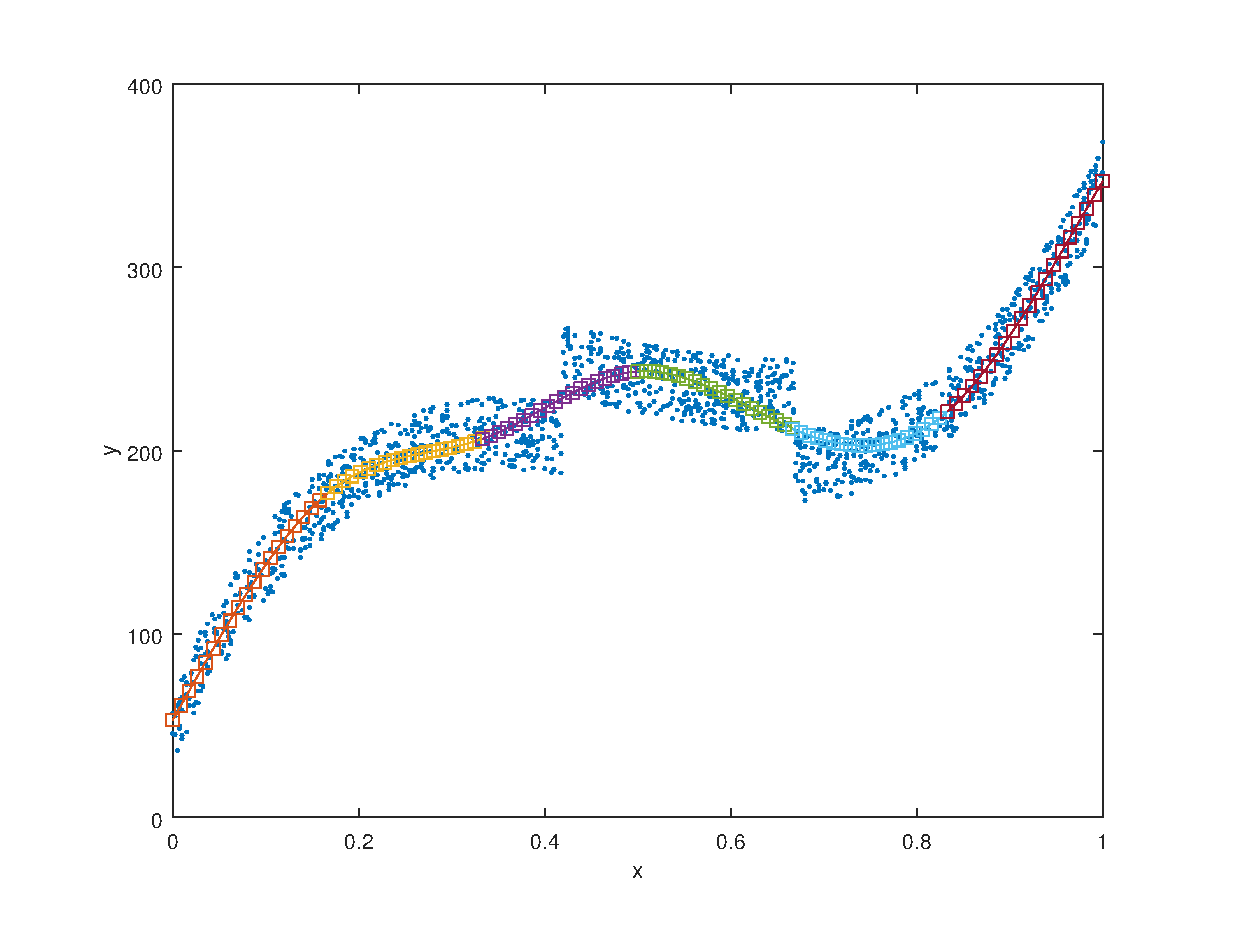
\includegraphics[scale=0.33]{splines3demo.eps}
\caption{Fitting of $M=6$ cubic splines in a set of $N=500$ pontos $(x_n,y_n)$.}
\label{fig:leastmeanspline3}
\end{figure}

Os splines tem seus limites de domínio, nas posições onde $x$ tem valores 
$\varepsilon_{0}, \varepsilon_{1}, \varepsilon_{2}, ..., \varepsilon_{M}$. 


Assim, usando as variáveis 
$\mathbf{E}=\left(\begin{matrix}\varepsilon_0 & \varepsilon_1 & ...  & \varepsilon_{M}\end{matrix}\right)^T$ e
$\mathbf{P}=\left(\begin{matrix}P_0 & P_1 & ...  & P_{4M-1}\end{matrix}\right)^T$,
podemos definir as seguintes funções,
\begin{equation}
 G(x,a,b)= \left\{\begin{matrix}
1 & if &  a \leq x \leq b \\ 
0 & if & other~case
\end{matrix}\right.
\end{equation}
\begin{equation}
 S_k(x,\mathbf{P})=P_{4k}+P_{1+4k}~x+P_{2+4k}~x^2+P_{3+4k}~x^3,
\end{equation}
de modo que
\begin{equation}
 f(x,\mathbf{P},\mathbf{E})=\sum_{k=0}^{M-1} S_k(x,\mathbf{P})G(x,\varepsilon_{k},\varepsilon_{k+1})  
\end{equation}

\subsection{Calculando os parâmetros $P_j$}

Para poder calcular o vetor $\mathbf{P}=\left(\begin{matrix}P_0 & P_1 & P_2 & ...  & P_{4M-1}\end{matrix}\right)^T$, 
do problema spline descrito  na Seção \ref{sec:spline3method1}, 
podemos definir as seguintes equações:
\begin{equation}
\left(\begin{matrix}
\mathbf{Y} \\
\mathbf{0} \\
\mathbf{0} \\
\mathbf{0} 
\end{matrix}\right)
=\left(\begin{matrix}
\mathbf{A} \\
\mathbf{B}_0 \\
\mathbf{B}_1 \\
\mathbf{B}_2 
\end{matrix}\right) \mathbf{P}
\end{equation}


\end{document}
